\documentclass[hyperref=colorlinks]{beamer}
\mode<presentation>
\usetheme{iclpt}
\setbeamertemplate{navigation symbols}{}
\setbeamertemplate{headline}{
\begin{beamercolorbox}[leftskip=.2cm,rightskip=.2cm,topskip=.2cm,ht=1.1cm,dp=0.1cm,wd=\textwidth]{institute in head/foot}
  
\includegraphics[height=1cm]{icl.pdf}
  \hfill
  
\includegraphics[height=1cm]{../Pics/CMS-Color.pdf}
\end{beamercolorbox}
}
\setbeamertemplate{footline}{
\begin{beamercolorbox}[ht=.55cm,dp=0.4cm,wd=\textwidth,leftskip=.3cm]{author in head/foot}%
  \begin{minipage}[c]{5cm}%
    \usebeamerfont{author in head/foot}
    \insertshortauthor 
    \insertshorttitle
    \end{minipage}\hfill%
  \insertframenumber{} / \pageref{lastframe}
  \hfill
  \begin{minipage}{6cm}
    \hfill
  \end{minipage}
\end{beamercolorbox}%
}

\usepackage{color}
\usepackage{tabularx,colortbl}
\usepackage{graphicx}
\usepackage{pdfpages}
\usepackage{feynmp}
\DeclareGraphicsRule{*}{mps}{*}{}

\title{\vspace{-0.2cm} VBF Higgs to Invisible - Update}
\subtitle{AN-14-243\vspace{-0.7cm}}
\author[P. Dunne]{\underline{P. Dunne}} % A.M. Magnan and A. Nikitenko Joao Pela with \\ R. Aggleton, J. Brooke: Bristol \\ C.Asawangtrakuldee, Q.Li: Peking \\ P. Srimanobhas: Chulalongkorn \\ S. Kumar, K. Mazumdar: Mumbai}
\titlegraphic{
  \vspace{-0.7cm}
  %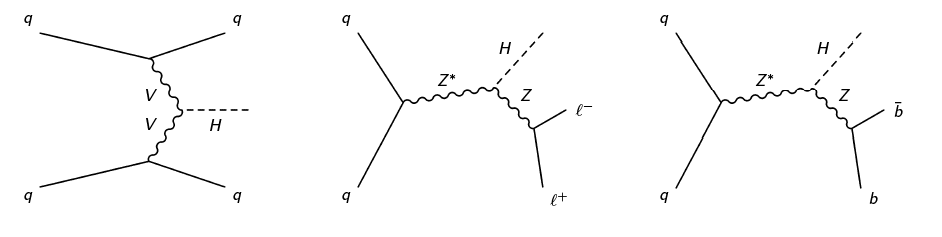
\includegraphics[width=\textwidth]{TalkPics/invcomb021213/feyndiags}
  %% \begin{fmfgraph*}(100,70)
  %%         \fmfleft{i1,i2}
  %%         \fmfright{o1,o2,o3}
  %%         \fmf{fermion}{i1,v1,o1}
  %%         \fmf{fermion}{i2,v2,o3}
  %%         \fmf{phantom,tension=4/5}{v1,v2}
  %%         \fmffreeze
  %%         \fmf{photon,label=$W,,Z$}{v1,v3}
  %%         \fmf{photon,label=$W,,Z$}{v2,v3}
  %%         \fmf{dashes}{v3,o2}
  %%         \fmflabel{$q$}{i1}
  %%         \fmflabel{$q$}{i2}
  %%         \fmflabel{$q$}{o1}
  %%         \fmflabel{$q$}{o3}
  %%         \fmflabel{$H$}{o2}
  %%       \end{fmfgraph*}
}
\date{}
\begin{document}
\begin{fmffile}{higgsexoupdatefeyndiags}

%TITLE PAGE
\section{Title}
\begin{frame}
  \titlepage
  
\end{frame}

%OUTLINE
\begin{frame}
  \frametitle{Introduction}
  \begin{block}{}
    \scriptsize
    \begin{itemize}
    \item Light trees have been made using prompt data ntuples and trigger weights
    \item Data cards have been made using the prompt light trees for both the prompt and parked cuts
    \item[-] I don't have the ggH samples or UES information in the prompt data ntuples,
    \item[-] ggH and UES are therefore neglected in all limits on next slide
    \item Results on next slide
    \item nb As we now drop $W\gamma$ the limits on the next slide should be compared to 46.29\% not the 49\% in the paper
    \end{itemize}
  \end{block}
\end{frame}

\begin{frame}
  \frametitle{Limits}
  \vspace{-.3cm}
  \begin{columns}
    \column{1.05\textwidth}
  \begin{block}{}
    \scriptsize
    \begin{itemize}
    \item $14\pm10$ used for parked cuts QCD estimate
    \item $31\pm23$ from paper used for prompt cuts QCD estimate
    \item Data driven top control region used for both prompt and parked cuts
    \item Prompt trigger weights ignore correlations in turn on part of parked cut region
    \end{itemize}
  \end{block}
  \vspace{-.25cm}
  \begin{block}{}
    \scriptsize
    \centering
    \begin{tabular}{|l|c|c|}
      \hline
      & Prompt trigger & parked trigger \\
      \hline
      Prompt cuts & 45.12\% & 45.51\% \\
      Parked cuts & 47.07\% & 39.65\% \\
      \hline
    \end{tabular}
  \end{block}
  \vspace{-.25cm}
  \begin{block}{\scriptsize Interpretation}
    \scriptsize
    \begin{itemize}
    \item Prompt cuts limits $\sim$ same as old card with both prompt and parked trigger
    \item The parked cuts give a worse limit with prompt trigger than with parked trigger
    \item[-] i.e.  We can only use the parked cuts because of the parked trigger
    \item Also seen in parked cuts control region data yields, most higher with parked trigger
    \item[-] Where prompt trigger yield is larger prompt and parked yields are within stat. unc. of each other
    \end{itemize}
  \end{block}
  \end{columns}
\end{frame}

\begin{frame}
  \frametitle{Summary}
  \label{lastframe}
  \begin{block}{}
    \scriptsize
    \begin{itemize}
    \item Prompt cuts numbers from light tree framework compatible with old cards for prompt and parked triggers
    \item Improvement to limit seen from using parked analysis cuts is only possible because of parked trigger
    \item Adding ggH and UES contribution back into parked trigger with parked cuts card gives limit of 37\% as shown on Monday
    \end{itemize}
  \end{block}
\end{frame}

\begin{frame}
  \frametitle{Backup}
\end{frame}

\end{fmffile}
\end{document}
